\documentclass[xcoler=dvipsnames, aspectratio=169]{beamer}
\usepackage{3191Style}
\date{Homogeneous Systems}
\begin{document}
    \begin{frame}{Homogeneous Systems}
        \begin{definition}
            \rText{Homogeneous}: A system of equations is \bText{homogeneous} if it can be written
            in the form $A\vec{x}=\vec{0}$.
        \end{definition}
        \begin{example}
            \small
            \begin{columns}
                \column{.5\textwidth}
                \only<1->{
                    \begin{eqnarray*}
                        x_1 + x_2 &=& 1\\
                        x_1 - 4x_2&=& 0
                    \end{eqnarray*}
                }
                \iftoggle{showSolutions}{
                    \only<2->{
                        \rText{Not homogeneous!}
                    }
                }{}
                \column{.5\textwidth}
                \only<1->{
                    \begin{eqnarray*}
                        x_1 + x_2 &=& 0\\
                        x_1 - 4x_2&=& 0
                    \end{eqnarray*}
                }
                \iftoggle{showSolutions}{
                    \only<2->{
                        \rText{Yes it is homogeneous!}
                    }
                }{}
            \end{columns}
        \end{example}
        \pause\pause
        \begin{tcolorbox}
            Every homogeneous system has a \rText{trivial solution} where $\vec{x}=\vec{0}$.
        \end{tcolorbox}
    \end{frame}
    \begin{frame}{Nontrivial Solutions Existence}
        Recall that the system $A\vec{x} = \vec{b}$ for all $\vec{b}\in\R^m$ has:
        \pause
        \begin{itemize}
            \item A unique solution if $A$ has a pivot in every row\pause
            \item Infinite number of solutions if $A$ has a solution and at least one free variable
        \end{itemize}
        \pause
        \vspace{100pt}
        \begin{theorem}
            The homogeneous equation $A\vec{x}=\vec{0}$ has a nontrivial solution if and only if
            the solution set has at least one free variable.
        \end{theorem}
    \end{frame}
    \begin{frame}{Solution Sets of Consistent Systems}
        Find the solution set to the homogeneous system write in vector form (from lecture 4):
        \begin{alignat*}{4}
            x_1 &+& 3x_2 &-& 2x_3 &=& 0\\
            -2x_1 &-& 6x_2 &+& 4x_3 &=& 0
        \end{alignat*}
        \iftoggle{showSolutions}{
            \pause
            \[
                \aMat{ccc|c}{
                    1&3&-2&0\\
                    -2&-6&4&0
                }\pause\rightarrow\aMat{ccc|c}{
                    1&3&-2&0\\
                    0&0&0&0
                }
            \]
            \pause
            This gives us:
            $x_1 = -3x_2 + 2x_3$ or as a vector:\pause
            \[
                \vec{x} = \begin{bmatrix}
                    x_1\\x_2\\x_3
                \end{bmatrix} \pause = \begin{bmatrix}
                    -3x_2+2x_3\\
                    x_2\\x_3
                \end{bmatrix} \pause = x_2\begin{bmatrix}
                    -3\\1\\0
                \end{bmatrix} + x_3\begin{bmatrix}
                    2\\0\\1
                \end{bmatrix} \pause = s\begin{bmatrix}
                    -3\\1\\0
                \end{bmatrix} + t\begin{bmatrix}
                    2\\0\\1
                \end{bmatrix}
            \]
        }{
            \vspace{140pt}
        }
    \end{frame}
    \begin{frame}{More Practice!}
        \small
        Find the solution set to the \bText{nonhomogeneous} system
        \begin{alignat*}{4}
            x_1 &+& 3x_2 &+& 7x_3 &=& 4\\
                &\,&x_2 &+& 3x_3 &=& 5\\
            -2x_1 &-& 4x_2 &-& 8x_3 &=& 2
        \end{alignat*}
        \iftoggle{showSolutions}{
            \pause
            \[
                \aMat{ccc|c}{
                    1&3&7&4\\
                    0&1&3&5\\
                   -2&-4&-8&2
                }\pause\rightarrow\aMat{ccc|c}{
                    1&3&7&4\\
                    0&1&3&5\\
                    0&2&6&10
                }\pause\rightarrow\aMat{ccc|c}{
                    1&3&7&4\\
                    0&1&3&5\\
                    0&0&0&0
                }\pause\rightarrow\aMat{ccc|c}{
                    1&0&-2&-11\\
                    0&1&3&5\\
                    0&0&0&0
                }
            \]
            Which can be written as
            \[
                \vec{x} = \begin{bmatrix}
                    x_1\\x_2\\x_3
                \end{bmatrix}\pause = \begin{bmatrix}
                    -11+2x_3\\5-3x_3\\x_3
                \end{bmatrix}\pause = \begin{bmatrix}
                    -11\\5\\0
                \end{bmatrix} + x_3\begin{bmatrix}
                    2\\-3\\1
                \end{bmatrix}\pause = \vec{p} + t\vec{v} (t\in\R)
            \]
        }{
            \vspace{120pt}
        }
    \end{frame}
    \begin{frame}{Comparing Homogeneous and Nonhomogeneous Solutions}
        \small
        \begin{columns}
            \column{.5\textwidth}
        \begin{alignat*}{4}
            x_1 &+& 3x_2 &+& 7x_3 &=& 0\\
                &\,&x_2 &+& 3x_3 &=& 0\\
            -2x_1 &-& 4x_2 &-& 8x_3 &=& 0
        \end{alignat*}
            \iftoggle{showSolutions}{
                \onslide<2->
                \vspace{-10pt}
                \[
                    \vec{x} = x_3\begin{bmatrix}
                    2\\-3\\1
                    \end{bmatrix} = t\vec{v} (t\in\R)
                \]
                \onslide<1->
            }{}
            \column{.5\textwidth}
        \begin{alignat*}{4}
            x_1 &+& 3x_2 &+& 7x_3 &=& 4\\
                &\,&x_2 &+& 3x_3 &=& 5\\
            -2x_1 &-& 4x_2 &-& 8x_3 &=& 2
        \end{alignat*}
            \iftoggle{showSolutions}{
                \onslide<2->
                \vspace{-10pt}
                \[
                    \vec{x} = \begin{bmatrix}
                        -11\\5\\0
                    \end{bmatrix} + x_3\begin{bmatrix}
                        2\\-3\\1
                    \end{bmatrix}= \vec{p} + t\vec{v} (t\in\R)
                \]
                \onslide<1->
            }{}
        \end{columns}
        \pause
        \iftoggle{showSolutions}{
            \pause
            \begin{center}
                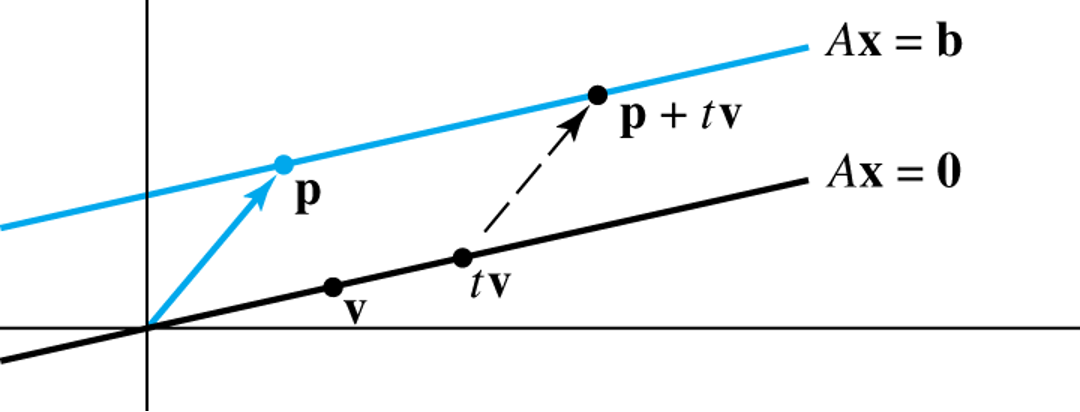
\includegraphics[width=3in]{./images/fig-translate.png}
            \end{center}
        }{}
    \end{frame}
    \begin{frame}{Infinite Solutions from Homogeneous System}
        \small
        \begin{theorem}
            Let $A\vec{x}=\vec{b}$ be a consistent system with solution $\vec{x}=\vec{p}$. Then
            there exists a solution set of vectors of the form
            \[
                \vec{x} = \vec{p} + t\vec{v}.
            \]
            Where $t\vec{v}$ is a solution to the \rText{homogeneous} system $A\vec{x} = \vec{0}$.
        \end{theorem}
        \pause
        \begin{proof}
            We will show this by showing $A\vec{x} = A\left(\vec{p} + t\vec{v}\right) = b$.
            \pause
            \begin{eqnarray*}
                A\vec{x} &=& A\left(\vec{p} + t\vec{v}\right)\pause \\ 
                &=& A\vec{p} + A(t\vec{v})\pause \\
                &=& \vec{b} + \vec{0}\pause\\
                &=& \vec{b}
            \end{eqnarray*}
        \end{proof}
    \end{frame}
\end{document}
